\documentclass{llncs}

\usepackage[utf8]{inputenc}
\usepackage[english]{babel}

\usepackage{amsmath,amsfonts,amssymb}
\usepackage{array}
\usepackage{url}

\usepackage{tikz,pgfplots}

\tikzset{
  baseline=(current bounding box.center)
}

\newcommand{\doctype}{Sample Sort with TBB}

\usepackage{hyperref}
\hypersetup{
  breaklinks=true,
  colorlinks=true,
  citecolor=blue,
  linkcolor=blue,
  urlcolor=blue,
  bookmarksnumbered,
  bookmarksopen,
  pdftitle={\doctype},
  pdfauthor={Michael Axtmann},
  pdfsubject={},
  pdfkeywords={},
}

% Final Submit TODO: remove following line which makes margins smaller
\hypersetup{pdfpagescrop={92 62 523 748}}

\usepackage{breakurl}

\title{\doctype}
\author{Damir Ferizovic, David Vogelbacher}
\institute{	Karlsruhe Institute of Technology, Karlsruhe, Germany\\
	\email{\{damir.ferizovic, david.vogelbacher\}@kit.edu}}


\begin{document}

%% sp-process: load data in sql-table 'stats'
% IMPORT-DATA stats ../run.log

\def\iterationcnt{10}

\maketitle

\begin{abstract}
We benchmark our implementation of the parallel sample sort algorithm using the Intel TBB framework \footnote{https://www.threadingbuildingblocks.org/}. We also compare it with the STL sort algorithm. 
\end{abstract}

% Final Submit TODO: remove this prior to FINAL submission
\pagestyle{plain}

\section{Algorithm - Sample Sort}
Let $p$ be the number of available threads. At the beginning of the sample sort algorithm, the input data is divided into $p$ groups ($p$ being the number of available threads) by using multiple pivot elements (similar to Quicksort). Then, each thread sorts one of the groups locally. The end result is just the concatenation of the local results.  In order to split the input, $p-1$ pivot elements are selected and the elements of the input are grouped into $p$ groups according to these pivot elements. Then, each thread sorts one of the groups. In order to get good pivot elements, oversampling is used: Initially, more than $S\cdot p$ elements are selected randomly as possible pivot elements for a constant $S$. These elements are then sorted (sequentially because the number of these elements is still small). After that, every $S$th element is selected as pivot element. This oversampling helps finding good pivot elements, such that the resulting groups are are of similar size with high probability.

\section{Inplementation Details}

\subsection{Pivot selection}
We randomly select $S \cdot p$ elements as possible pivot elements, where $S=4\cdot \frac{\log m}{0.1^2}$ ($m$ is the size of the input). We chose the value $S$ according to the lecture \footnote{http://algo2.iti.kit.edu/sanders/courses/paralg15/}. The value of $0.1$ for the parameter $\varepsilon$ was found to be quite good but other, similar values work as well. \\
We then sort the possible pivot elements using the sequential STL sorting algorithm (for large inputs with a large number of possible pivot elements one could recursively use sample sort). Lastly, we select every $S$th element as pivot element.
\subsection{Grouping of elements}
First, we calculate the group of each element by executing a \emph{parallel-for-loop} over the number of elements. Each iteration of the for-loop calculates the group to which the element belongs. We also store the element in a two-dimensional ThreadLocal array, where the first dimension is for each group and the second for the different elements of the group. \\
Second, using a \emph{parallel-for-loop} over the number of threads, each thread calculates the number of elements that belong to its group by looping over all arrays that were previously stored thread locally and summing the amount of elements that belong to its group.  \\
Lastly, each thread moves the elements belonging to its group into the right place in the original array. Elements of group $i$ are stored beginning at index  $\sum_{j=0}^{i-1}\text{groupsize}[j]$. Thus, after this step the original array is reordered in a way that elements belonging to the same group are stored next to each other.
\subsection{Local sorting}
As a last step, we sort all groups locally using the STL sorting algorithm and are finished.
\section{Experimental Results}
\subsection{Hardware}
\begin{itemize}
	\item OS: Linux (3.18.27-1-MANJARO)
	\item Processor: Intel(R) Core(TM) i7-3740QM CPU @ 2.70GHz with 4 cores and 8 threads
	\item RAM: 16GB
	\item Compiler: g++ (GCC) 5.3.0
\end{itemize}

\subsection{Experiments}
We benchmarked our implementation of sample sort and the STL sort using combinations of the following parameters:
\begin{itemize}
	\item Type of elements to be sorted: 32-bit Integer or 32-bit float
	\item Generator for elements: Either random or all zero
	\item Number of threads: 1,2,4,8
	\item Number of elements: From $10^5$ to $10^8$ in magnitudes of $10$
\end{itemize}

\subsection{Plots}

Running time~\ref{fi:runningtime:uniform} and speedup plots~\ref{fi:speedup:uniform} (for each generator, 64-bit integer and 32-bit floating point (not for  non-comparative integer sorting algorithms).

Interpretation.

\begin{figure}[h!]
\centering
\pgfplotsset{compat=1.5}
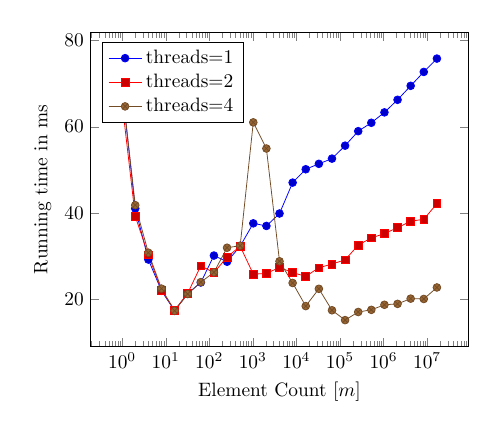
\begin{tikzpicture}[scale=0.7]
  \begin{axis}[
    xlabel={Element Count [$m$]},
    ylabel={Running time in ms},
    legend pos=north west,
    xmode=log,
    log basis x={10},
    ] 
    %% MULTIPLOT(threads) SELECT size AS x, time AS y, MULTIPLOT
    %% FROM stats
    %% WHERE "algo"='sample_sort' AND "generator"='random' AND "elementtype"='int'
    %% GROUP BY MULTIPLOT,x ORDER BY MULTIPLOT,x
    \addplot coordinates { (1,68.9184) (2,41.051) (4,29.2245) (8,21.9923) (16,17.3635) (32,21.3559) (64,23.9168) (128,30.1534) (256,28.718) (512,32.3257) (1024,37.6145) (2048,37.0117) (4096,39.8958) (8192,47.0518) (16384,50.1463) (32768,51.4022) (65536,52.608) (131072,55.6079) (262144,58.9654) (524288,60.9108) (1048576,63.3207) (2097152,66.2327) (4194304,69.4725) (8388608,72.6896) (16777216,75.779) };
    \addlegendentry{threads=1};
    \addplot coordinates { (1,65.449) (2,39.2551) (4,30.2806) (8,22.1556) (16,17.5) (32,21.4107) (64,27.7793) (128,26.1878) (256,29.7938) (512,32.3103) (1024,25.8488) (2048,25.9984) (4096,27.4117) (8192,26.1937) (16384,25.3417) (32768,27.3201) (65536,28.1916) (131072,29.1522) (262144,32.5654) (524288,34.2473) (1048576,35.2319) (2097152,36.6229) (4194304,38.1059) (8388608,38.5562) (16777216,42.1755) };
    \addlegendentry{threads=2};
    \addplot coordinates { (1,68.9796) (2,41.8265) (4,30.8112) (8,22.4923) (16,17.3571) (32,21.2519) (64,23.985) (128,26.2626) (256,31.9619) (512,32.4381) (1024,61.0072) (2048,54.9473) (4096,28.8268) (8192,23.8018) (16384,18.4491) (32768,22.4511) (65536,17.478) (131072,15.1969) (262144,17.0806) (524288,17.5748) (1048576,18.7493) (2097152,18.9607) (4194304,20.1748) (8388608,20.0965) (16777216,22.7603) };
    \addlegendentry{threads=4};
  \end{axis}
\end{tikzpicture}
\caption{Running times of \texttt{std::sort} and sample sort for random input of type Integer. Mean of \iterationcnt~iterations.}
\label{fi:runningtime:random"}
\end{figure}


\begin{figure}[h!]
\centering
\pgfplotsset{compat=1.5}
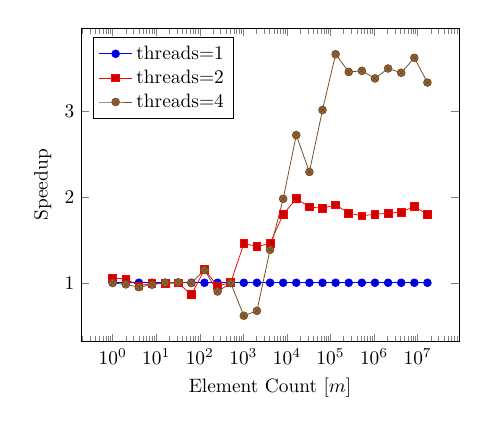
\begin{tikzpicture}[scale=0.7]
  \begin{axis}[
    xlabel={Element Count [$m$]},
    ylabel={Speedup},
    legend pos=north west,
    xmode=log,
    log basis x={10},
    ] 
    %% MULTIPLOT(threads) SELECT s.size AS x, s1.time / s.time AS y, s.threads
    %% FROM stats s CROSS JOIN stats s1
    %% WHERE 
    %% AND s."elementtype"='int'
    %% AND s."elementtype" = s1."elementtype"
    %% AND s."generator"='random'
    %% AND s."generator" = s1."generator"
    %% AND s.size = s1.size
    %% AND s1.threads=1
    %% GROUP BY s.threads,x ORDER BY s.threads,x
    \addplot coordinates { (1,1.0) (2,1.0) (4,1.0) (8,1.0) (16,1.0) (32,1.0) (64,1.0) (128,1.0) (256,1.0) (512,1.0) (1024,1.0) (2048,1.0) (4096,1.0) (8192,1.0) (16384,1.0) (32768,1.0) (65536,1.0) (131072,1.0) (262144,1.0) (524288,1.0) (1048576,1.0) (2097152,1.0) (4194304,1.0) (8388608,1.0) (16777216,1.0) };
    \addlegendentry{threads=1};
    \addplot coordinates { (1,1.05301) (2,1.04575) (4,0.965122) (8,0.992631) (16,0.992201) (32,0.997438) (64,0.860956) (128,1.15143) (256,0.963889) (512,1.00048) (1024,1.45518) (2048,1.42361) (4096,1.45543) (8192,1.7963) (16384,1.9788) (32768,1.88148) (65536,1.86608) (131072,1.9075) (262144,1.81068) (524288,1.77856) (1048576,1.79725) (2097152,1.8085) (4194304,1.82315) (8388608,1.88529) (16777216,1.79675) };
    \addlegendentry{threads=2};
    \addplot coordinates { (1,0.999112) (2,0.981459) (4,0.948501) (8,0.97777) (16,1.00037) (32,1.00489) (64,0.997155) (128,1.14815) (256,0.898506) (512,0.996537) (1024,0.616558) (2048,0.673586) (4096,1.38398) (8192,1.97682) (16384,2.71809) (32768,2.28951) (65536,3.00995) (131072,3.65916) (262144,3.45219) (524288,3.46581) (1048576,3.37722) (2097152,3.49315) (4194304,3.44354) (8388608,3.61703) (16777216,3.32945) };
    \addlegendentry{threads=4};
  \end{axis}
\end{tikzpicture}
\caption{Speedup of \texttt{std::sort} with uniform input. Mean of \iterationcnt~iterations.}
\label{fi:speedup:random:int}
\end{figure}


%\bibliographystyle{splncs03}
%\bibliography{/home/axtman/promotion/latex/library}

\end{document}
